\chapter{Summary and Outlook}
\label{ch:summary}

\dictum[Charles Darvin]{%
   I am turned into a sort of machine for observing facts and grinding out conclusions. }
\vskip 1em


The continental subsurface plays a fundamental role in global environmental processes, including carbon sequestration, long-term nuclear waste storage, and geothermal energy production.
As interest in deep subsurface reservoirs continues to expand, there is a growing need to improve our understanding of fluid dynamics, geochemical interactions, and microbial ecosystems in these environments.
Geothermal systems provide particularly valuable natural laboratories for studying these interactions, as they represent environments where deep fluid circulation, microbial life, and geological activity are tightly linked.
However, numerous fundamental questions concerning the stability, adaptability, and geochemical influence of these systems persist, particularly in relation to seismic activity and hydrological variations.

This thesis sought to address these challenges by investigating fluid-seismic interactions and deep microbial ecosystems in the Lavey-les-Bains geothermal system in Switzerland.
The research was conducted by integrating geochemical monitoring, isotopic analysis, long-term high-resolution dissolved gas measurements, and microbial DNA sequencing.
The results of this study have provided insights into microbial stability at depth, the dominance of temperature in shaping microbial ecosystems, and the potential of geochemical signals in deep thermal waters as indicators of water quality in response to seismic activity.
Beyond its site-specific relevance, this thesis contributes to broader discussions on microbial adaptation in extreme environments and deep groundwater evolution.

\section*{Microbial Ecosystems and Their Broader Implications}
A significant finding of this study is the remarkable stability of deep geothermal microbial communities, even in the presence of seasonal hydrological variations and geochemical fluctuations.
This suggests that these ecosystems are primarily structured by thermal gradients rather than transient changes in fluid chemistry.
While this stability has been well characterized, the functional activity of these microbes remains largely unknown.

Future studies should shift focus toward resolving microbial metabolic activity and ecological functions, particularly their contributions to global elemental cycling and deep subsurface geochemistry.
Metagenomic and metatranscriptomic analyses hold considerable potential to reveal active metabolic pathways in geothermal conditions, such as carbon fixation, sulfur and nitrogen cycling, and methane metabolism.
These processes are essential for understanding how geothermal microbial communities influence the geochemical evolution of deep subsurface environments.

In addition, incubation experiments could complement sequencing-based approaches by providing direct constraints on microbial metabolic rates, physiological limits, and generation times, while also enabling the measurement of enzymatic activities linked to major biogeochemical transformations.
A combined approach, integrating genomic, transcriptomic, and physiological studies, would allow for a more complete understanding of microbial persistence and evolution in extreme geothermal environments and their contributions to global biogeochemical cycles.

Beyond their ecological role, these microbial communities may serve as biosensors for environmental perturbations in subsurface reservoirs.
Given their minimal seasonal variation, sudden shifts in microbial composition or metabolic function could serve as indicators of seismic activity, fault activation, or fluid migration within geothermal reservoirs.
Regular microbial monitoring (e.g., BactoSense\textsuperscript{\tiny\textregistered}) could complement geochemical and geophysical monitoring, contributing to early-warning systems for large subsurface environmental changes.

\subsection*{Advancing Long-Term Geochemical Monitoring}
A key outcome of this research is the advancement of long-term gas monitoring strategies using the miniRUEDI system.
One major challenge in geothermal gas monitoring is that, when water temperatures exceed ambient conditions, water vapor can condense within the gas phase, leading to clogging and interruptions in monitoring.
This study developed a mitigation strategy for geothermal waters, which has since been applied to other groundwater monitoring projects, particularly in colder climates where groundwater temperatures exceed ambient air temperatures in winter.

Beyond these technical improvements, long-term gas monitoring has revealed short-term geochemical variations correlated with regional seismic activity.
These findings suggest that elastic deformation of subsurface pore structures and pressure changes influence groundwater mixing ratios, potentially serving as precursors to seismic events.
While the observed effects were localized and hydrogeologically dependent, this study provides one of the first long-term records of geochemical responses to seismicity in a deep continental geothermal system.
To refine this approach, future work should focus on:

\begin{itemize}
    \item Expanding the range of gas tracers used in seismic monitoring (e.g., \ce{H2S}, \ce{H2}),
    \item Investigating depth resolution by deploying multi-level monitoring systems within geothermal reservoirs,
    \item Assessing the time lag between geochemical fluctuations and seismic events to evaluate their predictive potential in earthquake monitoring.
\end{itemize}

\section*{Expanding the Scope: Applications Beyond Lavey-les-Bains}
While this study was conducted in Lavey-les-Bains, its methodologies and findings have global applicability to other tectonically active geothermal regions.
Similar research in Iceland, the Apennines (Italy), the San Andreas Fault (USA), New Zealand, and Japan could test the reproducibility of these findings and refine geochemical monitoring to assess water quality in response to seismicity.
Additionally, integrating geochemical and microbial monitoring in diverse geothermal fields could improve understanding of subsurface fluid dynamics, microbial adaptation, and geothermal resource evolution.

Beyond investigating the relationship between water quality and seismicity, this research has advanced helium-based geothermal prospecting (Figure~\ref{fig:concl_valais}), demonstrating that elevated \ce{^4He} concentrations can serve as tracers for deep geothermal reservoirs. 
Excess non-atmospheric \ce{^4He} in shallow groundwater provides evidence of deep groundwater intrusion, as such water is naturally enriched with terrigenic helium.
However, further research is needed to refine spatial resolution, assess helium diffusion effects, and explore the feasibility of detecting helium in surface gas emissions within the unsaturated zone.
Future work should focus on multi-scale testing of helium tracing and integrating geophysical data to better constrain subsurface fluid migration and reservoir connectivity.

\FloatBarrier  

\begin{figure}[t]  % Allow some flexibility in placement
\begin{center}
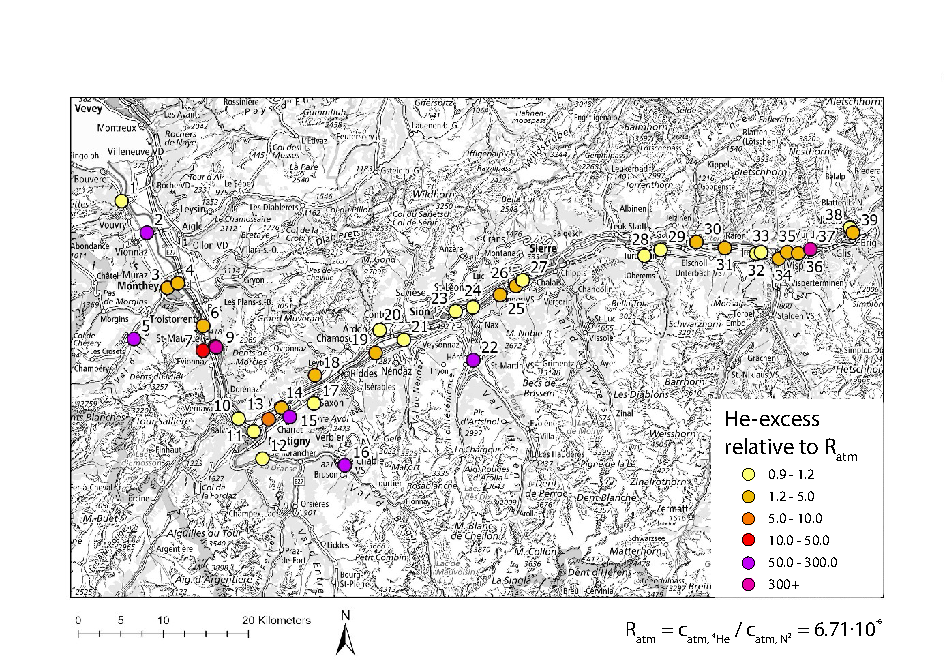
\includegraphics[width=0.9\textwidth]{chapters/05_conclusion_outlook/valais.pdf}
\end{center}
\caption{Helium sampling campaign in the Canton of Valais.
A total of 39 locations were sampled to assess \ce{^4He} concentrations and their enrichment patterns within the water table.
Adapted from \cite{marion2023valais}.}
\label{fig:concl_valais}
\end{figure}

\FloatBarrier  % Ensure no floats move past this point

\section*{Concluding Remarks}
By addressing knowledge gaps in geothermal fluid-seismic interactions and deep microbial ecosystems, this thesis presents a new framework for high-resolution monitoring in hydrothermal environments.
As long-term monitoring technologies continue to evolve, interdisciplinary studies integrating geochemistry, microbiology, and geophysics will be essential in refining our understanding of deep Earth processes and their global significance.
These efforts will support more sustainable geothermal resource management, improved seismic risk assessment, and new insights into microbial life in extreme environments.